\documentclass[
size=17pt,
paper=smartboard,
mode=present,
display=slidesnotes,
style=sailor,
nopagebreaks,
blackslide,
fleqn]{powerdot}
 %wj capsules prettybox
 %mode = handout or present

\usepackage{amsmath,graphicx,color}
\usepackage[brazilian]{babel}
\usepackage[utf8]{inputenc}


\author{Ronaldo de Freitas Zampolo\\FCT-ITEC-UFPA}
\date{ }


\pdsetup{
   lf = {\cursopequeno},
   rf = {Introdução ao projeto de filtros},
   cf = {\theslide},
   palette = \palette,
   randomdots={false}
}
\title{\cursogrande\\ \vspace{1cm}Introdução do projeto de filtros}

\begin{document}
\maketitle[randomdots={false}]
   \begin{slide}{Agenda}
      \tableofcontents[content=sections]
   \end{slide}

\section{Introdu\c c\~ao}

\begin{slide}{Introdu\c c\~ao}
\begin{itemize}
   \item Etapas de um projeto de filtros:
   \begin{itemize}
      \item Definição das especificações de um filtro: suas características desejáveis
      \item Aproximação: definição de uma função de transferência ou resposta ao impulso que atenda às especificações
      \item Realização: implementação usando uma determinada estrutura ou sistema
   \end{itemize}
\end{itemize}
\end{slide}

\section{Especificações de um filtro}
%\begin{slide}{Especificações de um filtro passa-baixas}
%\begin{itemize}
%   \item Filtro passa-baixas ideal
%   \begin{equation}
%      H_{lp}(e^{j\omega})\begin{cases}e^{-j\alpha \omega}, & |\omega |\leq \omega_c \\
%                                                                0, & \omega_c < | \omega | \leq \pi \end{cases}
%   \end{equation}
%   \begin{itemize}
%      \item Supondo que um sinal de entrada $x[n]$ seja limitado em freqüência e esteja todo contido na banda passante de um filtro passa-baixas ideal, qual a saída $y[n]$?
%      \item Mostre que a resposta ao impulso unitário de um filtro passa-baixas ideal é 
%   \begin{equation}
%      h_{lp}[n] = \frac{\text{sen}[\omega_c(n-\alpha)]}{\pi(n-\alpha)} = \frac{\omega_c}{\pi}\text{sinc}\left [ \frac{\omega_c(n-\alpha)}{\pi}\right ] 
%   \end{equation}
%   \end{itemize}
%\end{itemize}
%\end{slide}

%\begin{slide}{Especificações de um filtro passa-baixas}
%\begin{itemize}
%   \item Filtro passa-baixas ideal: resposta ao impulso \\($\omega_c = \pi/16$ rad)\\
%   \includegraphics[width = 0.85\textwidth]{figs/h_16.eps}
%\end{itemize}
%\end{slide}
%
%\begin{slide}{Especificações}
%\begin{itemize}
%   \item Filtro passa-baixas ideal: resposta ao impulso \\($\omega_c = \pi/8$ rad)\\
%   \includegraphics[width = 0.85\textwidth]{figs/h_8.eps}
%\end{itemize}
%\end{slide}
%
%\begin{slide}{Especificações}
%\begin{itemize}
%   \item Filtro passa-baixas ideal: resposta ao impulso \\($\omega_c = \pi/4$ rad)\\
%   \includegraphics[width = 0.85\textwidth]{figs/h_4.eps}
%\end{itemize}
%\end{slide}
%
%\begin{slide}{Especificações}
%\begin{itemize}
%   \item Filtro passa-baixas ideal: resposta ao impulso \\($\omega_c = \pi/2$ rad)\\
%   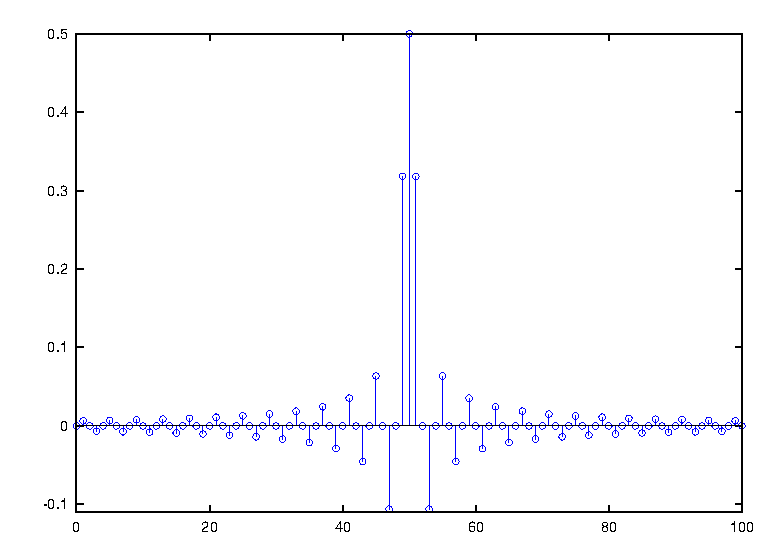
\includegraphics[width = 0.85\textwidth]{figs/h_2.eps}
%\end{itemize}
%\end{slide}

%\begin{slide}{Especificações}
%\begin{itemize}
%   \item Filtro passa-baixas ideal: resposta ao impulso \\($\omega_c = \pi$ rad)\\
%   \includegraphics[width = 0.85\textwidth]{figs/h_1.eps}
%\end{itemize}
%\end{slide}


%\begin{slide}{Especificações}
%\begin{itemize}
%   \item Filtro passa-baixas ideal
%   \begin{itemize}
%      \item Exercício: Determine a resposta ao impulso dos filtros passa-altas, passa-banda e rejeita-banda ideais
%   \end{itemize}
% \end{itemize}
%\end{slide}
%
%
\begin{slide}{Filtros realizáveis}
\begin{itemize}
   \item Como a resposta ao impuso de filtros ideais é irrealizável, as especificações devem ser mais \emph{relaxadas}:
   \begin{figure}
	   \centering
	   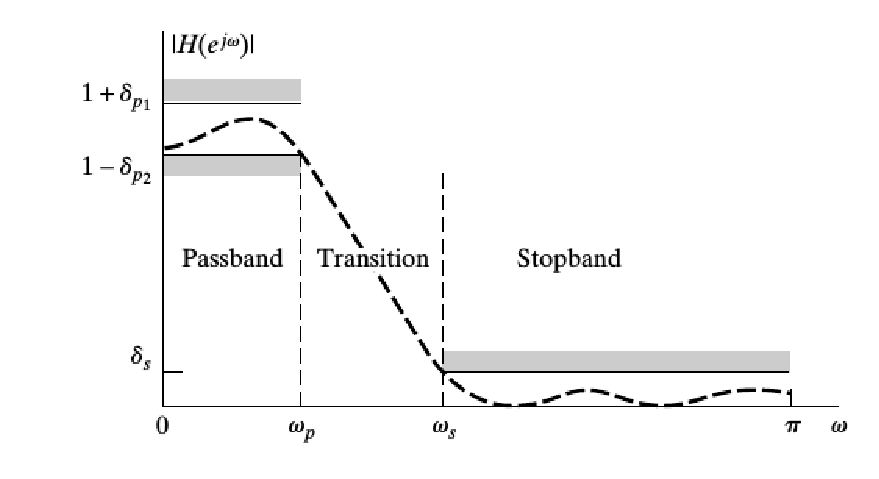
\includegraphics[width = 0.8\textwidth]{figs/specifications.eps}
   \end{figure}
\end{itemize}
\end{slide}

\section{Projeto de filtros IIR} 
\begin{slide}{Projeto de filtros IIR discretos a partir de filtros contínuos}
	\begin{itemize}
		\item Procedimento geral:
			\begin{itemize}
				\item As especificações do filtro efetivo são determinadas	
				\item As especificações do filtro discreto são mapeadas
				\item As especificações de um filtro contínuo protótipo são calculadas
				\item O projeto do filtro protótipo é realizado, usando alguma técnica de aproximação
				\item O filtro discreto é determinado a partir do filtro protótipo
				\item São comparadas as características do filtro projetado com os requisitos de projeto
			\end{itemize}
	\end{itemize}
\end{slide}

\begin{slide}{Método da invariância da resposta ao impulso}
	\begin{itemize}
		\item A resposta ao impulso do filtro discreto é obtida por amostragem da resposta ao impulso do filtro protótipo projetado:
			\begin{align*}
				h[n] &= T_dh_c(nT_d)\\
				H(e^{j\omega}) &= H_c\left( j\frac{\omega}{T_d}\right ), \qquad |\omega|\leq \pi
			\end{align*}
		\item Normalmente a resposta em frequência do filtro protótipo não é limitada em banda:
			\begin{figure}
				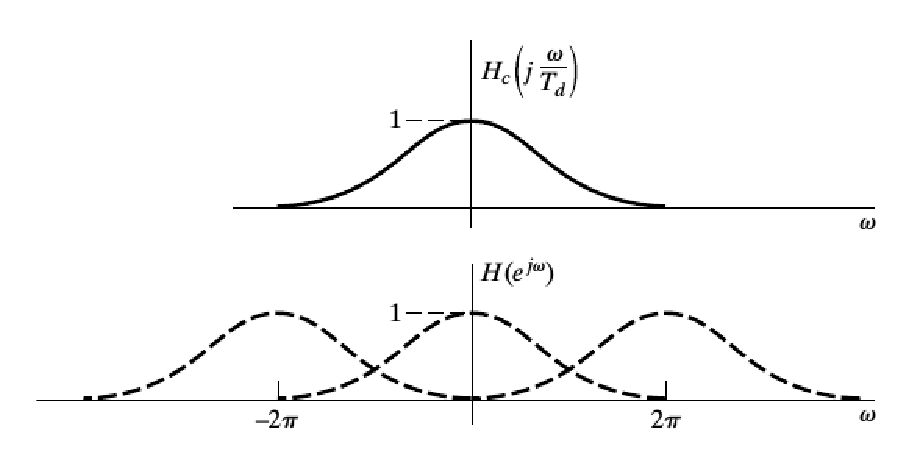
\includegraphics[width = 0.5\textwidth]{figs/impulse-invariance.eps}
			\end{figure}
	\end{itemize}
\end{slide}

\begin{slide}{Método da invariância da resposta ao impulso}
	\begin{itemize}
		\item Passo a passo:
		\begin{itemize}
			\item Especificações do filtro discreto
			\item Especificações do filtro protótipo contínuo
			\item Projeto do filtro protótipo, ou seja, obtenção de $H_c(s)$
			\item Determinação de $H(z)$ a partir de $H_c(s)$:
			\begin{itemize}
				\item Transformada inversa de $H_c(s)$, ou seja, $h_c(t)$ (mais fácil se expandir em frações parciais a partir deste ponto)
				\item Cálculo de $h[n] = T_dh_c(nTd)$
				\item Determinação de $H(z)$, mediante o cálculo da transformada Z de $h[n]$
			\end{itemize}
		\end{itemize}
	\end{itemize}
\end{slide}

\begin{slide}{Método da invariância da resposta ao impulso}
	\begin{itemize}
		\item Relação entre pares de trasformada de Laplace
			\begin{align*}
				Ae^{s_kt}u(t) &\rightarrow \frac{A}{s-s_k}
			\end{align*}
		\item Relação entre pares de transformada Z
			\begin{align*}
				T_dA(e^{s_kT_d})^nu[n] &\rightarrow \frac{T_dA}{1-e^{s_kT_d}z^{-1}}
			\end{align*}
	\end{itemize}
\end{slide}

%\begin{slide}{Método da invariância da resposta ao impulso}
%	\begin{minipage}{\textwidth}
%	\begin{minipage}{0.5\textwidth}
%		\begin{itemize}
%			\item Especificações do filtro contínuo
%				\begin{align*}
%					\delta_{p1} &= \delta_{p2} = 1\text{ dB}\\
%					\delta_s    &= -60\text{ dB}\\
%					f_p &= 2,5 \text{ kHz}\\
%					f_s &= 3,0 \text{ kHz}\\
%					f_a &= 8 \text{ kHz}
%				\end{align*}
%		\end{itemize}
%		\end{minipage}
%	\begin{minipage}{0.5\textwidth}
%		\begin{itemize}
%			\item Especificações do filtro discreto
%				\begin{align*}
%					\delta_{p1} &= \delta_{p2} = 1\text{ dB}\\
%					\delta_s    &= -60\text{ dB}\\
%					\omega_p &= \frac{f_p}{f_a}2\pi = \frac{2,5}{8}2\pi \text{ rad}\\
%					\omega_s &= \frac{f_s}{f_a}2\pi \frac{3,0}{8}2\pi \text{ rad}\\
%					%f_s &= 8 \text{ kHz}
%				\end{align*}
%		\end{itemize}
%		\end{minipage}
%	\end{minipage}
%	\begin{minipage}{0.9\textwidth}
%		\begin{itemize}
%			\item Especificações do filtro protótipo contínuo
%				\begin{align*}
%					\delta_{p1} &= \delta_{p2} = 1\text{ dB} &&\delta_s= -60\text{ dB}\\
%					f_p^p &= \frac{f_p}{f_a} f_d = \frac{2,5}{8} f_d \text{ kHz} && f_s^p=\frac{f_s}{f_a} f_d= \frac{3,0}{8} f_d \text{ kHz}\\
%					f_d &= 16 \text{ kHz}
%				\end{align*}
%		\end{itemize}
%	\end{minipage}
				%\item Especificações do filtro discreto:
				%\item Especificações do filtro protótipo:
				%\item Filtro protótipo obtido:
				%\item Filtro discreto final:
				%\item Verificação das especificações:
			%\end{itemize}
%\end{slide}

\begin{slide}{Transformação bilinear}
	\begin{itemize}
		\item Substituição de variável: \begin{equation*} s = \frac{2}{T_d}\left ( \frac{1-z^{-1}}{1+z^{-1}}\right )\end{equation*}
		\item Passo a passo:
		\begin{itemize}
			\item Especificações do filtro discreto
			\item Especificações do filtro protótipo contínuo
			\item Projeto do filtro protótipo, ou seja, obtenção de $H_c(s)$
			\item Determinação de $H(z)$ a partir de $H_c(s)$, usando a transformação bilinear
		\end{itemize}
	\end{itemize}
\end{slide}

\begin{slide}{Exemplos comparativos}
	\begin{itemize}
		\item Especificações do filtro
			\begin{itemize}
				\item $\omega_p = 0,5\pi$
				\item $\omega_s = 0,6\pi$
				\item $\delta_{p1} = 0$ dB
				\item $\delta_{p2} = -0,3$ dB
				\item $\delta_{s} = -30$ dB
			\end{itemize}
		\item Aproximações:
			\begin{itemize}
				\item Butterworth
				\item Chebyshev I
				\item Chebyshev II
				\item Elíptico
			\end{itemize}
	\end{itemize}
\end{slide}

\begin{slide}{Magnitude da resposta em frequência}
	\begin{itemize}
		\item Butterworth
			\begin{figure}
				\centering 
				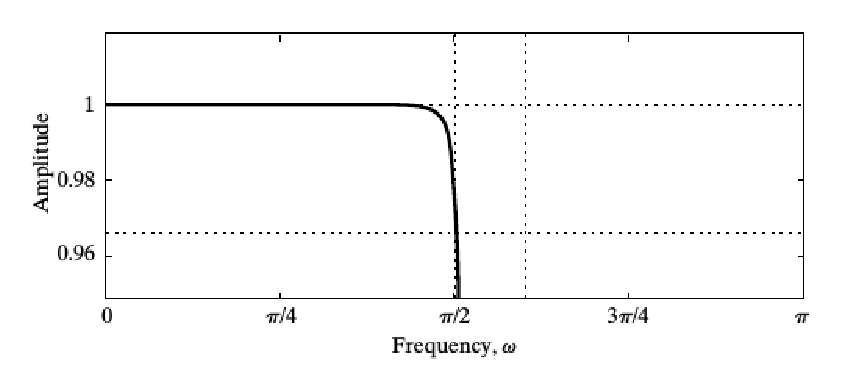
\includegraphics[width = 0.45\textwidth]{figs/bmag.eps}
			\end{figure}
		\item Chebyshev I
			\begin{figure}
				\centering 
				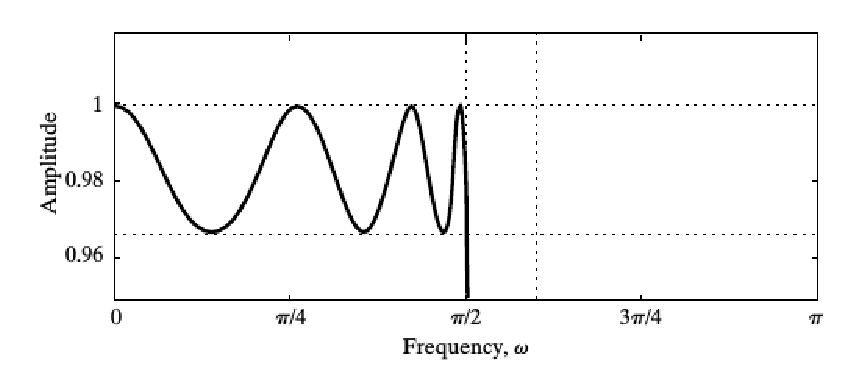
\includegraphics[width = 0.45\textwidth]{figs/cmag.eps}
			\end{figure}
	\end{itemize}
\end{slide}
\begin{slide}{Magnitude da resposta em frequência}
	\begin{itemize}
		\item Chebyshev II
			\begin{figure}
				\centering 
				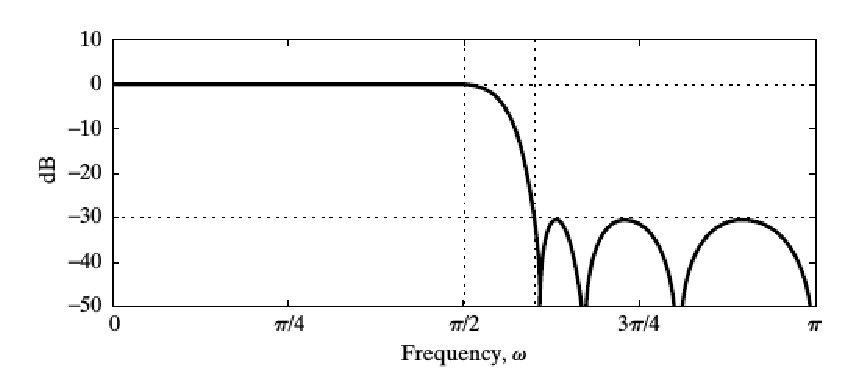
\includegraphics[width = 0.45\textwidth]{figs/c2mag.eps}
			\end{figure}
		\item Elíptico
			\begin{figure}
				\centering 
				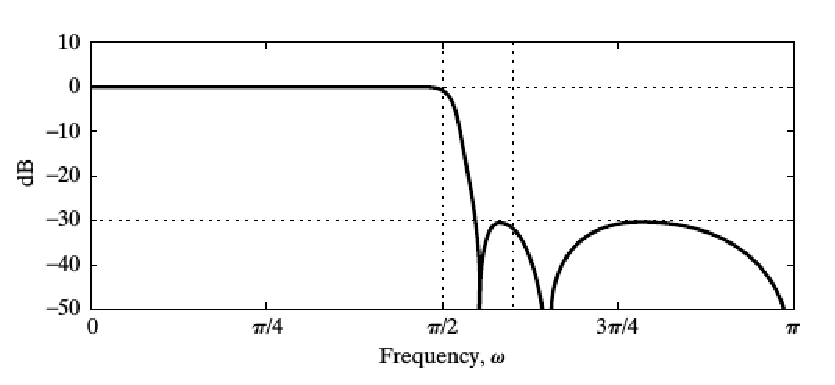
\includegraphics[width = 0.45\textwidth]{figs/emag1.eps}
				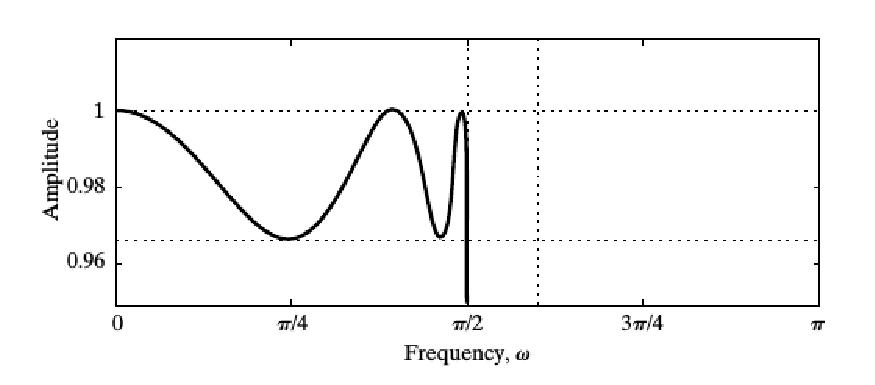
\includegraphics[width = 0.45\textwidth]{figs/emag2.eps}
			\end{figure}
	\end{itemize}
\end{slide}

\begin{slide}{Diagrama de polos e zeros}
	\begin{itemize}
		\item Butterworth
			\begin{figure}
				\centering 
				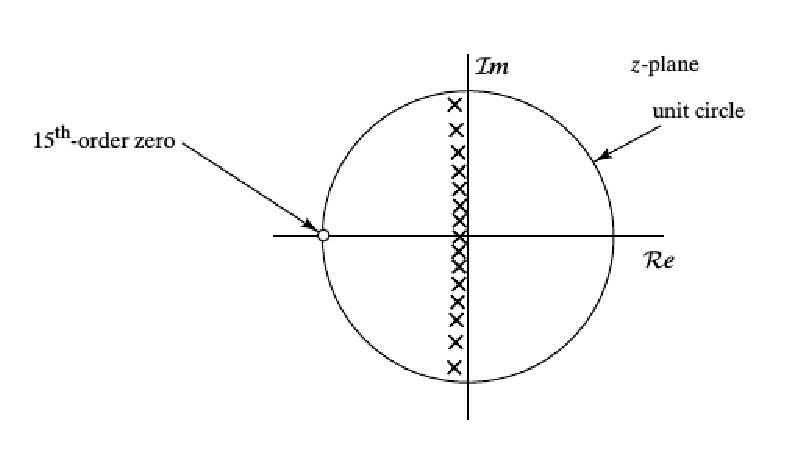
\includegraphics[width = 0.35\textwidth]{figs/bpz.eps}
			\end{figure}
		\item Chebyshev I
			\begin{figure}
				\centering 
				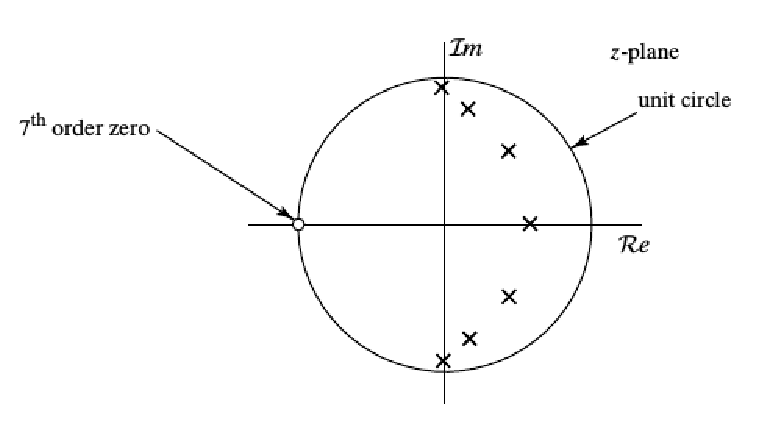
\includegraphics[width = 0.35\textwidth]{figs/cpz.eps}
			\end{figure}
	\end{itemize}
\end{slide}
\begin{slide}{Diagrama de polos e zeros}
	\begin{itemize}
		\item Chebyshev II
			\begin{figure}
				\centering 
				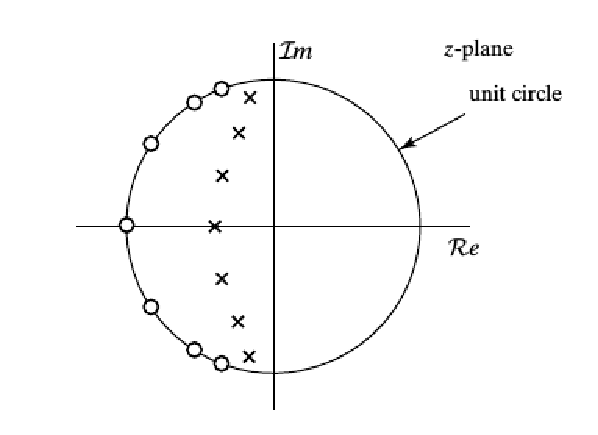
\includegraphics[width = 0.25\textwidth]{figs/c2pz.eps}
			\end{figure}
		\item Elíptico
			\begin{figure}
				\centering 
				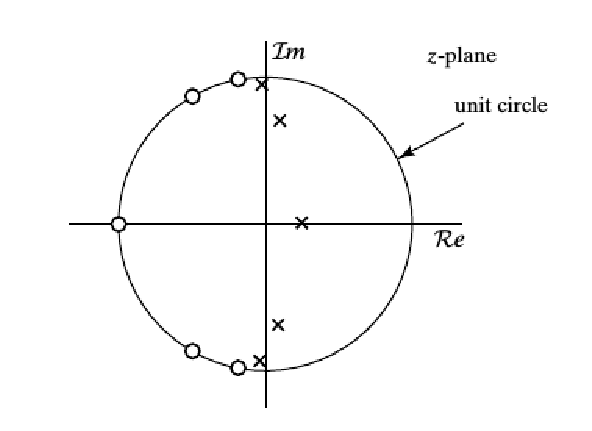
\includegraphics[width = 0.25\textwidth]{figs/epz.eps}
			\end{figure}
	\end{itemize}
\end{slide}



\section{Projeto de filtros FIR} 
\begin{slide}{Projeto de Filtros FIR}
\begin{itemize}
   \item Projeto de filtros FIR de fase linear usando janelas 
   \begin{equation}
      h[n] = h_d[n]w[n]
   \end{equation}
   \begin{itemize}
      \item $h[n]$: coeficientes do filtro FIR (resposta ao impulso)
      \item $h_d[n]$: resposta ao impulso do filtro ideal
      \item $w[n]$: função-janela 
      \begin{itemize}
         \item $w[n]=0$, fora do intervalo $0\leq n\leq N$
         \item $w[n] = w[N-n]$
     \end{itemize}
   \end{itemize}
\end{itemize}
\end{slide}

\begin{slide}{Projeto de Filtros FIR}
\begin{itemize}
   \item Projeto de filtros FIR de fase linear usando janelas 
   \begin{equation}
      h[n] = h_d[n]w[n]
   \end{equation}
   \begin{itemize}
      \item No domínio da freqüência,
      \begin{align}
        H(e^{j\omega}) &= \frac{1}{2\pi}H_d(e^{j\omega})\ast W(e^{j\omega})\\
                                   &= \frac{1}{2\pi}\int_{-\pi}^{\pi}H_d(e^{j\theta})W(e^{j(\omega-\theta)}) d\theta
      \end{align}
     \textcolor{red}{O janelamento \emph{suavisa} a resposta em freqüência dos filtros ideais.}
   \end{itemize}
\end{itemize}
\end{slide}

\begin{slide}{Projeto de Filtros FIR}
\begin{itemize}
   \item Projeto de filtros FIR de fase linear usando janelas 
   \begin{itemize}
      \item Fatores que influenciam a degradação da resposta em freqüência
      \begin{itemize}
         \item Largura do lobo principal de $W(e^{j\omega})$: quanto menor melhor
         \item Amplitude relativa de pico dos lobos secundários $W(e^{j\omega})$: quanto menor melhor
      \end{itemize}
      \item Largura do lobo principal: diminui com o aumento do tamanho da janela (dualidade seqüência/freqüência)
      \item Amplitude de pico dos lobos secundários: depende da forma da janela
   \end{itemize}
\end{itemize}
\end{slide}

\begin{slide}{Projeto de Filtros FIR}
\begin{itemize}
   \item Projeto de filtros FIR de fase linear usando janelas 
   \begin{itemize}
      \item Exemplo: Janela retangular com $N=5$
      \includegraphics[width=0.6\textwidth]{figs/w_ret_5.eps}
   \end{itemize}
\end{itemize}
\end{slide}

\begin{slide}{Projeto de Filtros FIR}
\begin{itemize}
   \item  Projeto de filtros FIR de fase linear usando janelas 
   \begin{itemize}
      \item Exemplo: Janela retangular com $N=10$
      \includegraphics[width=0.6\textwidth]{figs/w_ret_10.eps}
   \end{itemize}
\end{itemize}
\end{slide}

\begin{slide}{Projeto de Filtros FIR}
\begin{itemize}
   \item  Projeto de filtros FIR de fase linear usando janelas 
   \begin{itemize}
      \item Exemplo: Janela retangular com $N=100$
      \includegraphics[width=0.6\textwidth]{figs/w_ret_100.eps}
   \end{itemize}
\end{itemize}
\end{slide}

\begin{slide}{Projeto de Filtros FIR}
\begin{itemize}
   \item  Projeto de filtros FIR de fase linear usando janelas 
   \begin{itemize}
      \item Janelas mais usadas:
      \begin{itemize}
         \item Janela retangular
         \begin{equation*}
            w[n] = \begin{cases}1,&0\leq n\leq N\\ 0,& \text{outro caso}\end{cases}
         \end{equation*}
       \end{itemize}
   \end{itemize}
\end{itemize}
\includegraphics[width=0.45\textwidth]{figs/wn_ret_10.eps}
\includegraphics[width=0.45\textwidth]{figs/w_ret_10.eps}
\end{slide}

\begin{slide}{Projeto de Filtros FIR}
\begin{itemize}
   \item  Projeto de filtros FIR de fase linear usando janelas 
   \begin{itemize}
      \item Janelas mais usadas:
      \begin{itemize}
         \item Janela de Hann
         \begin{equation*}
            w[n] = \begin{cases}0,5-0,5\cos\left ( \frac{2\pi n}{N}\right ),&0\leq n\leq N\\ 0,& \text{outro caso}\end{cases}
         \end{equation*}
       \end{itemize}
   \end{itemize}
\end{itemize}
\includegraphics[width=0.45\textwidth]{figs/wn_han_10.eps}
\includegraphics[width=0.45\textwidth]{figs/w_han_10.eps}
\end{slide}

\begin{slide}{Projeto de Filtros FIR}
\begin{itemize}
   \item  Projeto de filtros FIR de fase linear usando janelas 
   \begin{itemize}
      \item Janelas mais usadas:
      \begin{itemize}
         \item Janela de Hamming
         \begin{equation*}
            w[n] = \begin{cases}0,54-0,46\cos\left ( \frac{2\pi n}{N}\right ),&0\leq n\leq N\\ 0,& \text{outro caso}\end{cases}
         \end{equation*}
       \end{itemize}
   \end{itemize}
\end{itemize}
\includegraphics[width=0.45\textwidth]{figs/wn_ham_10.eps}
\includegraphics[width=0.45\textwidth]{figs/w_ham_10.eps}
\end{slide}

\begin{slide}{Projeto de Filtros FIR}
\begin{itemize}
   \item  Projeto de filtros FIR de fase linear usando janelas 
   \begin{itemize}
      \item Janelas mais usadas:
      \begin{itemize}
         \item Janela de Blackman
         \begin{equation*}
            w[n] = \begin{cases}0,42-0,5\cos\left ( \frac{2\pi n}{N}\right ) + 0,08\cos\left ( \frac{4\pi n}{N}\right ),&0\leq n\leq N\\ 0,& \text{outro caso}\end{cases}
         \end{equation*}
       \end{itemize}
   \end{itemize}
\end{itemize}
\includegraphics[width=0.45\textwidth]{figs/wn_bla_10.eps}
\includegraphics[width=0.45\textwidth]{figs/w_bla_10.eps}
\end{slide}

\begin{slide}{Projeto de Filtros FIR}
\begin{itemize}
   \item  Projeto de filtros FIR de fase linear usando janelas 
   %\scriptsize{
   \begin{tabular}{c|p{8cm}|c|p{8cm}}
      \hline\hline
      Janela & Amplitude do lobo secundário & $\Delta f$ & Atenuação~na banda de rejeição\\
      \hline\hline
      Retangular & -13 dB & 0,9/N & -21 dB\\
      Hanning     & -31 dB & 3,1/N & -44 dB \\
      Hamming  & -41 dB  & 3,3/N & -53 dB\\
      Blackman  & -57 dB & 5,5/N & -74 dB\\
      \hline\hline
   \end{tabular}%}
   \begin{itemize} 
      \item Exercício: Projete um filtro FIR de fase linear que atenda às seguintes especificações
      \begin{equation*}\begin{cases}
         0,99\leq |H(e^{j\omega})| \leq 1,01 & 0\leq |\omega| \leq 0,19\pi\\
          |H(e^{j\omega})| \leq 0,01 & 0,21\pi\leq |\omega| \leq \pi
          \end{cases}
       \end{equation*}
   \end{itemize}
\end{itemize}
\end{slide}

\begin{slide}{Projeto de Filtros FIR}
\begin{itemize}
   \item  Projeto de filtros FIR de fase linear usando janelas 
   \begin{itemize} 
      \item Exercício (cont.)\\
      Atenuação na banda de rejeição:
      \begin{equation*}
         \delta_s = 20\log_{10}(0,01) =  -40 \text{ dB}
      \end{equation*}
      Banda de Transição:
      \begin{align*}
         \Delta_f &= \frac{\Delta_\omega}{2\pi}\\ &= \frac{\omega_s -\omega_p}{2\pi}\\&= \frac{0,21\pi - 0,19\pi}{2\pi}\\&=0,01
      \end{align*}
   \end{itemize}
\end{itemize}
\end{slide}

\begin{slide}{Projeto de Filtros FIR}
\begin{itemize}
   \item  Projeto de filtros FIR de fase linear usando janelas 
   \begin{itemize} 
      \item Exercício (cont.)\\
      Comprimento da janela (Hann)
      \begin{align*}
         N &= \frac{3,1}{\Delta_f}\\
            &= 310
      \end{align*}
      Freqüência de corte ($\omega_c$) e atraso ($\alpha$):
      \begin{align*}
         \omega_c &= \frac{\omega_s + \omega_p}{2}= 0,2\pi\\
         \alpha       &=\frac{N}{2}= 155
      \end{align*}
   \end{itemize}
\end{itemize}
\end{slide}

\begin{slide}{Projeto de Filtros FIR}
\begin{itemize}
   \item  Projeto de filtros FIR de fase linear usando janelas 
   \begin{itemize} 
      \item Exercício (cont.)\\
      Substituir $\omega_c$, e $\alpha$ em
      \begin{align*}
         h_d[n] &= \frac{sen[\omega_c(n-\alpha)]}{\pi(n-\alpha)} = \frac{\omega_c}{\pi}sinc\left [ \frac{\omega_c(n-\alpha)}{\pi}\right ] \\
       \end{align*}
      Calcular a janela $w[n]$, usando $N$
   \end{itemize}
\end{itemize}
\end{slide}

\begin{slide}{Projeto de Filtros FIR}
\begin{itemize}
   \item  Projeto de filtros FIR de fase linear usando janelas 
   \begin{itemize}
      \item Exercício (cont.)
    \end{itemize}
\end{itemize}
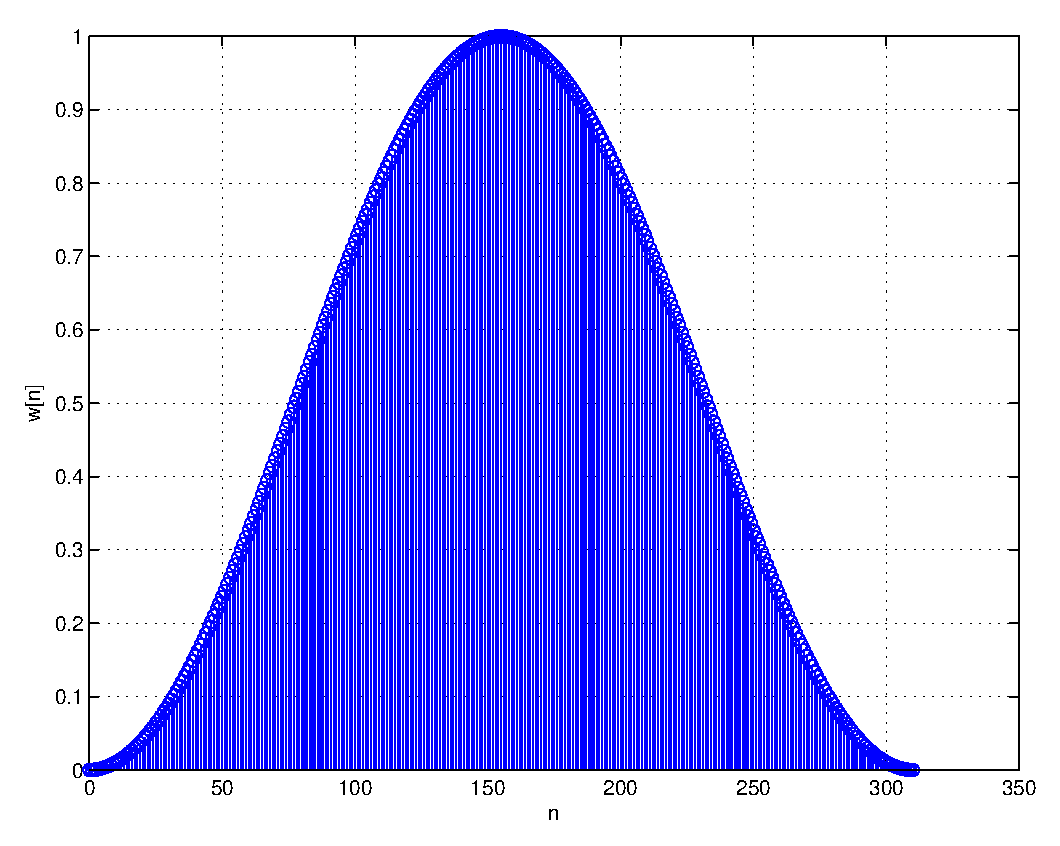
\includegraphics[width=0.6\textwidth]{figs/janela.eps}
%\includegraphics[width=0.48\textwidth]{ideal.eps}
\end{slide}

\begin{slide}{Projeto de Filtros FIR}
\begin{itemize}
   \item  Projeto de filtros FIR de fase linear usando janelas 
   \begin{itemize}
      \item Exercício (cont.)
    \end{itemize}
\end{itemize}
\includegraphics[width=0.6\textwidth]{figs/ideal.eps}
%\includegraphics[width=0.48\textwidth]{janelada.eps}
\end{slide}

\begin{slide}{Projeto de Filtros FIR}
\begin{itemize}
   \item  Projeto de filtros FIR de fase linear usando janelas 
   \begin{itemize}
      \item Exercício (cont.)
    \end{itemize}
\end{itemize}
%\includegraphics[width=0.7\textwidth]{ideal.eps}
\includegraphics[width=0.6\textwidth]{figs/janelada.eps}
\end{slide}


\begin{slide}{Projeto de Filtros FIR}
\begin{itemize}
   \item  Projeto de filtros FIR de fase linear usando janelas 
   \begin{itemize}
      \item Exercício (cont.)
    \end{itemize}
\end{itemize}
\includegraphics[width=0.55\textwidth]{figs/H.eps}
%\includegraphics[width=0.48\textwidth]{Hdb.eps}
\end{slide}

\begin{slide}{Projeto de Filtros FIR}
\begin{itemize}
   \item  Projeto de filtros FIR de fase linear usando janelas 
   \begin{itemize}
      \item Exercício (cont.)
    \end{itemize}
\end{itemize}
%\includegraphics[width=0.48\textwidth]{H.eps}
\includegraphics[width=0.55\textwidth]{figs/Hdb.eps}
\end{slide}

\begin{slide}{Projeto de Filtros FIR}
\begin{itemize}
   \item  Projeto de filtros FIR de fase linear usando janelas 
   \begin{itemize}
      \item Janela de Kaiser
      \begin{equation*}
          w[n] = \begin{cases}
                  \frac{I_0\{\beta[1-(n-\alpha)^2/\alpha^2]^{1/2}}{I_0(\beta)}, & 0\leq n\leq N\\
                  0, & \text{outro caso}
                 \end{cases}
      \end{equation*}
      onde $I_0(x)$ \'e a fun\c c\~ao de Bessel modificada de ordem zero, que pode ser determinada pela expans\~ao
      \begin{equation*}
          I_0(x) = 1+\sum_{k=1}^{\infty}\left [ \frac{(x/2)^k}{k!}\right ]^2
      \end{equation*}
      
   \end{itemize}
\end{itemize}
%\includegraphics[width=0.48\textwidth]{H.eps}
%\includegraphics[width=0.7\textwidth]{Hdb.eps}
\end{slide}

\begin{slide}{Projeto de Filtros FIR}
\begin{itemize}
   \item  Projeto de filtros FIR de fase linear usando janelas 
   \begin{itemize}
      \item Janela de Kaiser (Etapas de projeto)
      \begin{itemize}
         \item Deteminar a atenua\c c\~ao na banda de rejei\c c\~ao:
         \begin{equation*}
            \alpha_s = -20\log_{10}(\delta_s)
         \end{equation*}
         \item Calcular $\beta$
      \end{itemize}    
   \end{itemize}
\end{itemize}
\begin{equation*}
            \beta =\begin{cases}
                       0,1102(\alpha_s-8,7) & \alpha_s>50\\
                       0,5842(\alpha_s-21)^{0,4}+0,07886(\alpha_s-21) & 21\leq \alpha_s\leq 50\\
                       0,0 & \alpha_s<21
                   \end{cases}
         \end{equation*}
%\includegraphics[width=0.48\textwidth]{H.eps}
%\includegraphics[width=0.7\textwidth]{Hdb.eps}
\end{slide}

\begin{slide}{Projeto de Filtros FIR}
\begin{itemize}
   \item  Projeto de filtros FIR de fase linear usando janelas 
   \begin{itemize}
      \item Janela de Kaiser (Etapas de projeto)
      \begin{itemize}
         \item Determinar o valor de $N$
         \begin{equation*}
            N = \begin{cases}
                 \frac{\alpha_s-7,95}{14,36\Delta_f} & \alpha_s\geq 21\\
                 \frac{0,9}{\Delta_f} & \alpha_s<21
                \end{cases}
         \end{equation*}
      \end{itemize}    
   \end{itemize}
\end{itemize}
%\includegraphics[width=0.48\textwidth]{H.eps}
%\includegraphics[width=0.7\textwidth]{Hdb.eps}
\end{slide}

%\section{Projeto de filtros usando mínimos quadrados} 

\end{document}
